\documentclass[16pt]{article}
\usepackage[russian]{babel}
\usepackage{a4wide}
\usepackage[utf8]{inputenc}
\usepackage{graphicx}
\usepackage{amsmath}
\usepackage{amssymb}
\usepackage{amsthm}
\usepackage{import}
\usepackage{xifthen}
\usepackage{pdfpages}
\usepackage{transparent}

\newcommand{\incfig}[2]{%
    \def\svgwidth{#2 mm}
    \import{./figures/}{#1.pdf_tex}
}

\newtheorem{Th}{Теорема}
\newtheorem{Lem}{Лемма}
\newenvironment{Proof}{\par\noindent{\bf Доказательство.}}{\hfill$\scriptstyle\blacksquare$}
\newenvironment{Sol}{\par\noindent{\it Решение:}}


\DeclareMathOperator{\Arccos}{arccos}
\DeclareMathOperator{\Arctg}{arctg}
\DeclareMathOperator{\Cl}{Cl}
\DeclareMathOperator{\SI}{SI}
\DeclareMathOperator*{\Argmax}{Argmax}
\DeclareMathOperator*{\Var}{Var}
\DeclareMathOperator*{\Min}{min}


\newcommand\Real{\mathbb{R}} 
\newcommand\A{(\cdot)} 
\newcommand\Sup[2]{\rho( #1 \, | \, #2 )}
\newcommand\Sum[2]{\sum\limits_{#1}^{#2}}
\newcommand\Scal[2]{\langle #1,\, #2 \rangle}
\newcommand\Norm[1]{\left\| #1 \right\|}
\newcommand\Int[2]{\int\limits_{#1}^{#2}}
\newcommand\PS{\mathcal{P}}
\newcommand\X{\mathcal{X}} 
\newcommand\Pict[3]{
\begin{figure}[h!]
    \centering
    \incfig{#1}{#3}
    \caption{#2}
    \label{fig:#1}
\end{figure}
}

\begin{document}

\thispagestyle{empty}

\begin{center}
\ \vspace{-3cm}

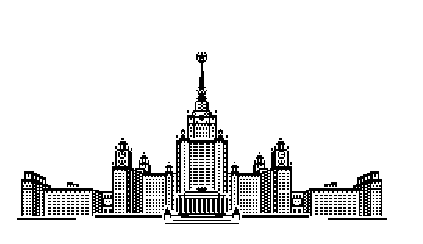
\includegraphics[width=0.5\textwidth]{msu.eps}\\
{\scshape Московский государственный университет имени М.~В.~Ломоносова}\\
Факультет вычислительной математики и кибернетики\\
Кафедра системного анализа

\vfill

{\LARGE Отчёт по самому важному предмету}

\vspace{1cm}

{\Huge\bfseries <<Задание 2 практикума по оптимальному управлению>>}
\end{center}

\vspace{1cm}

\begin{flushright}
  \large
  \textit{Студент 315 группы}\\
  Д.\,М.~Сотников

  \vspace{5mm}

  \textit{Руководитель практикума}\\
  к.ф.-м.н., доцент П.\,А.~Точилин
\end{flushright}

\vfill

\begin{center}
Москва, 2020
\end{center}

\newpage
\tableofcontents
\newpage
\part{Теоретическая часть}
\section{Постановка задачи}
Вертикальное движение ракеты описывается системой дифференциальных уравнений
\begin{equation}
\begin{cases} \label{task_ode}
\dot{m}v + m\dot{v} = -gm + lu \\
\dot{m} = -u
\end{cases}
\end{equation}
Здесь $v \in \Real$ --- скорость ракеты, $m$ --- масса ракеты, $g > 0$ --- гравитационная постоянная,
$l > 0$ --- коэффициент, определяющий силу, действующую на ракету со стороны сгорающего топлива,
$u \in [0, u_{max}]$ --- скорость подачи топлива, $u_{max} > 0$. Масса ракеты без топлива равна $M > 0$.
Если топливо заканчивается ($m = M$), то дивгатель ракеты отключается, то есть $u = 0$.

Заданы начальный момент $t_0 = 0$, начальная скорость $v(0) = 0$, начальная масса ракеты с топливом $m(0) = 
m_0 > M$. Движение ракеты описывается системой (\ref{task_ode}) на всем отрезке времени, движение вниз в 
начальный момент времени невозможно, то есть $v(t) > 0, \  t \in [0, \delta]$ для некоторого $\delta > 0$.
\paragraph{Задача 1.} 
Найти измеримое управление $u\A$, переводящее ракету на максимальную высоту~$H$ в заданный момент времени $T > 0$
 так, чтобы $v(T) \in [-\epsilon,\epsilon]$.

\paragraph{Задача 2.} Найти измеримое управление $u\A$, переводящее ракету на заданную высоту $H >~0$ в момент
 времени $T > 0$, минимизируя функционал
 $$ J = \Int{0}{T} u^4(t)dt.$$

\section{Преобразование системы}
Сделаем замену переменных $x_1(t) = v(t) + l, \ x_2(t) = m(t)$, а также подставим $\dot{m} = -u$
в первое уравнение системы (\ref{task_ode}) и поделим его на $m$.
В новых переменных система принимает вид
\begin{equation}
\begin{cases} \label{rocket_ode}
\dot{x}_1 = -g + \dfrac{x_1u}{x_2} \\
\dot{x}_2 = -u
\end{cases}
\end{equation}

Такое представление удобно, поскольку дает возможность решить систему аналитически при постоянных $u$.
\section{Ограничения на входные параметры}
Помимо явных ограничений на параметры ($g > 0, l > 0, u_{max} > 0$) в системе так же присутствует неявное
ограничение: как было указано в постановке задачи, для взлеты ракеты ее скорость должна стать положительной, 
для этого её производная $\dot{v} = \dot{x}_1$ должна быть положительна в начальный момент времени. 
Используя $x_1(0) = l, \ x_2(0) = m_0$, получим следующее ограничение на управление:
\begin{equation} \label{u0_restr}
u(0) \geqslant \dfrac{m_0g}{l}
\end{equation}
Отсюда же следует, что
$ u_{max} \geqslant \dfrac{m_0g}{l}.$ Если это неравенство не выполнено, будем считать задачу некорректно поставленной.

Из интерпретации следует, что параметр $\epsilon$ в задаче 1 мал, поскольку требуется практически остановить ракету
на максимально возможной высоте. А именно, пусть 
\begin{equation} \label{eps_restr}
\epsilon < l.
\end{equation}

\section{Вспомогательные утверждения}
\indent Главным утверждением, использующимся для решения задачи, является принцип максимума Понтрягина,
 доказательство которого когда-нибудь будет изложено в \cite{OC}. 
 
 Рассматривается задача оптимального управления автономной системой
 $$ \dot{x}(t) = f(x(t), u(t)), \quad t \in [t_0, t_1],\  x(t) \in \Real^n, \ u(t) \in \Real^m$$
  с минимизацией функционала
 $$J = \Int{t_0}{t_1}f_0(x(t), u(t))dt \to \inf_{u\A}$$
 из множества $\X_0$ в множество $\X_1$, то есть $x(t_0) \in \X_0, \ x(t_1) \in \X_1$. В классе измеримых
 управлений требуется найти $u\A$ такое, что $u(t) \in \PS(t)$ почти всюду на $[t_0, t_1]$ и $u\A$ является решением
 поставленной выше задачи. Здесь $\PS\A$ --- заданное измеримое многозначное отображение, $\PS(t)$ является выпуклым
 компактом при любом $t \in [t_0, t_1]$.
 
 Функционал Гамильтона-Понтрягина имеет вид
 $$\mathcal{H}(x, u, \tilde{\psi}) = \psi_0 f_0(x, u) + \Scal{\psi}{f(x, u)},$$
 где $\psi = (\psi_1, \ldots, \psi_n) \in \Real^n, \ \psi_0 \in \Real$.
\begin{Th}[Принцип максимума Понтрягина]
Пусть $(x^*\A, u^*\A)$ --- решение поставленной задачи оптимального управления. Тогда найдется 
$\tilde{\psi} = (\psi_0, \psi_1, \ldots, \psi_n), \ \tilde{\psi} \not\equiv 0$ такой, что  
$$\mathcal{H}(x^*(t), u^*(t), \tilde{\psi}(t)) \overset{\text{\rm п.в.}}{=} \max_{u \in \PS(t)} 
\mathcal{H}(x^*(t), u, \tilde{\psi}(t)).$$
При этом $\psi_0 \leqslant 0$ и постоянна, а $\psi(t)$ является решением сопряженной системы
$$ \dot{\psi}(t) = -\frac{\partial\mathcal{H}}{\partial x}(x^*(t), u^*(t), \tilde{\psi}(t)),$$
и выполнены условия трансверсальности 
$$\psi(t_0) \bot T_{x^*(t_0)}\X_0, \quad \psi(t_1) \bot T_{x^*(t_1)}\X_1.$$
\end{Th}

Рассмотрим так же несколько вспомогательных утверждений, относящихся к дифференциальным уравнениям.
\begin{Lem} Пусть функции $a\A, b\A$ непрерывны на $[t_0, t_1]$. Тогда задача Коши 
$$\dot{x}(t) = a(t)x(t) + b(t), \quad x(t_0) = x^0$$
имеет решение
$$ x(t) = x^0 e^{\Int{t_0}{t}a(s)ds} + \Int{t_0}{t} b(\tau)e^{\Int{\tau}{t}a(s)ds}d\tau.$$
\end{Lem}

\begin{Lem}
Пусть функции $a\A, b\A$ непрерывны на $[t_0, t_1]$ и $b\A$ знакопостоянна и не обращается в ноль на $[t_0, t_1]$.
Тогда решение уравнения $\dot{x}(t) = a(t)x(t) + b(t)$ обращается в ноль не более, чем в одной точке, возрастая в ее  окрестности, если $b > 0$, и убывая, если $b < 0$.
\end{Lem}
\begin{Proof}
Пусть, для определенности, $b(t) > 0$ при любых $t \in [t_0, t_1]$, и пусть решение уравнения обращается в 0
в точке $\tau \in [t_0, t_1]$. Тогда $\dot{x}(\tau) = b(\tau) > 0$, что также выполняется в маленькой окрестности точки $\tau$, поэтому функция $x\A$ возрастает этой окрестности.
Это означает, что траектория может пересекать ноль только <<снизу-вверх>>. Объединяя это с непрерывностью $x\A$,
получаем требуемое утверждение.
\end{Proof}

Договоримся для краткости, что запись $f > 0 \ (f < 0)$ означает положительность (отрицательность)
 функции почти всюду на рассматриваемом отрезке 
$[t_0,\,t_1]$.
\section{Решение задачи 1}
В координатах $(x_1, x_2)$ начальное и конечное множества имеют вид
$$\X_0 = \{l\} \times \{m_0\}, \quad \X_1 = [l-\epsilon, \, l+\epsilon] \times [M, \, m_0].$$
\Pict{1_X1}{Множество $\X_1$}{90}

Максимизация высоты $H(T) = \Int{0}{T}v(t)dt$ эквивалентна максимизации функционала $$J = \Int{0}{T}x_1(t)dt$$
Для данной задачи функционал Гамильтона-Понтрягина имеет вид 
$$\mathcal{H} = \psi_0x_1 + \psi_1(-g + \frac{x_1u}{x_2}) - \psi_2u = (\psi_0x_1 - \psi_1g) +
 (\frac{\psi_1x_1}{x_2} - \psi_2)u.$$

Введем вспомогательную функцию $F(t) = \psi_1(t)x_1(t) - \psi_2(t)x_2(t)$. Очевидно, что функционал 
Гамильтона-Понтрягина является возрастающей линейной функцией по $u$ тогда и только тогда, когда $F(t) > 0$.
Здесь мы воспользовались тем, что $x_2 > 0$ всюду на $[0,\,T]$.
 
 
Из условия максимума получаем, что 
 \begin{equation} \label{oc_1}
 u(t) = 
 \begin{cases}
 u_{max}, & F(t) > 0,\  x_2(t) > M, \\
 [0,\, u_{max}], & F(t) = 0, \ x_2(t) > M, \\
 0, &\text{иначе.}
 \end{cases}
 \end{equation}

Из условий трансверсальности и вида множества $\X_1$ следует, что $\psi_2(T) = 0$ при $x_2(T)\in~(M,\,m_0)$, и
$\psi_1(T) = 0$ при $x_2(T) = M$.

Заметим также, что $x_1(t) > 0$ всюду на $[0,\,T]$. Это следует из того, что $x_1(T) > l - \epsilon 
\overset{(\ref{eps_restr})}{>} 0$ и леммы 2: если найдется $\tau \in (0,\,T)$ такое, что $x_1(\tau) = 0$, 
то $x_1(t) < 0$ для всех $t > \tau$.

Рассмотрим теперь возможные режимы движения системы, которые будут получены из принципа максимума Понтрягина.
\subsection{Нормальный случай}
Пусть $\psi_0 \not = 0$. Тогда в силу положительной однородности принципа максимума по $\tilde{\psi}$ можно считать,
что $\psi_0 = 1$. Тогда сопряженная система имеет вид 
\begin{equation}
\begin{cases} \label{1_conj_sys1}
\dot{\psi}_1 = -\dfrac{\partial \mathcal{H}}{\partial x_1} = -1 + \dfrac{\psi_1u}{x_2}\\
\dot{\psi}_2 = -\dfrac{\partial \mathcal{H}}{\partial x_2} = \dfrac{\psi_1 x_1 u}{x_2^2}
\end{cases}
\end{equation}

Вычислим $\dot{F} = \dot{\psi}_1x_1 + \psi_1\dot{x}_1 - \dot{\psi}_2x_2 - \psi_2\dot{x}_2 = -x_1 +
\dfrac{\psi_1x_1u}{x_2} - \psi_1 g - \dfrac{\psi_1x_1u}{x_2} - \dfrac{\psi_1x_1u}{x_2} + \psi_2u = \\
=-x_1 - \psi_1g - \dfrac{Fu}{x_2}.$ Таким образом получили, что $F$ удовлетворяет дифференциальному уравнению
\begin{equation} \label{F_ode}
\dot{F} = (-x_1 - \psi_1g) - \dfrac{Fu}{x_2}.
\end{equation}
Рассмотрим теперь, как будут меняться режимы движения в зависимости от того, закончилось ли топливо к концу полета
или нет.
\paragraph{Случай $m(T) > M$}
Пусть к моменту времени $T$ было израсходавано не все топливо. Тогда из условий трансверсальности следует, что
$\psi_2(T) = 0$, а значит $F(T) = \psi_1(T)x_1(T)$. 

\subparagraph{Пусть $F(T) \geqslant 0$} Если $F(T) \geqslant 0$, то $\psi_1(T) \geqslant 0$, и, по лемме 2, 
$\psi_1 > 0$. Но тогда
$-x_1 -~\psi_1g <~0$, и из уравнения (\ref{F_ode}) и леммы 2 следует, что $F > 0$. Но это означает, что
$$u(t) = u_{max}, \quad t \in [0,\,T].$$

\subparagraph{Пусть $F(T) < 0$} В этом случае можно утверждать, что найдется точка $\tau_s$, в которой 
$F(\tau_s) = 0$, и $F(t) < 0, \ t \in (\tau_s,\,T]$. Если такой точки нет, то $F < 0$, и двигатель всегда 
будет выключен, что невозможно в поставленной задаче (ракета упадет на землю). Из вида управления (\ref{oc_1})
 следует, что $u(t) = 0, \ t > \tau_s$. Тогда, решая задачу Коши на $[\tau_s,\,T]$ получаем $\psi_2(\tau_s) = 0$.
Поскольку $F(\tau_s) = \psi_1(\tau_s)x_1(\tau_s) = 0$, получаем $\psi_1(\tau_s) = 0$. Далее рассуждениями, полностью
 аналогичными прошлому случаю, получаем $u(t) = u_{max}$ на $[0,\,\tau_s]$.
 
\paragraph{Случай $m(t) = M$}
Из условия трансверсальности $\psi_1(T) = 0$, откуда по лемме 2 $\psi_1 > 0$. Так как топливо закончилось, был
промежуток времени, в который двигатель был включен. Пусть $\tau_F$ --- момент, когда топливо закончилось, то есть
$F(\tau_F) \geqslant 0$. Заметим вновь, что $(-x_1 - \psi_1g) < 0$, и поэтому $F > 0,\ u = u_{max}$ 
на $[0,\,\tau_s]$. 

\paragraph{Вывод}
Подведем итог нормального случая. Все допустимые режимы имеют следующий вид: $u(t) = u_{max}$ до некоторого момента 
выключения двигателя либо до тех пор, пока не кончится топливо (то есть в момент $\tau_F = \dfrac{m_0-M}{u_{max}}$).
\subsection{Анормальный случай}
Пусть $\psi_0 = 0$. Тогда сопряженная система имеет вид
\begin{equation}
\begin{cases} \label{1conj_sys2}
\dot{\psi}_1 = -\dfrac{\partial \mathcal{H}}{\partial x_1} = \dfrac{\psi_1u}{x_2}\\
\dot{\psi}_2 = -\dfrac{\partial \mathcal{H}}{\partial x_2} = \dfrac{\psi_1 x_1 u}{x_2^2}
\end{cases}
\end{equation}
Фкнкция $F$ удовлетворяет дифференциальному уравнению
$$\dot{F} = -\psi_1g - \dfrac{Fu}{x_2}.$$

\paragraph{Случай $m(T) > M$} $F(T) = \psi_1(T)x_1(T)$. 
\subparagraph{Пусть $F(T) < 0$} $\psi_1(T) < 0$, поэтому из сопряженной системы $\psi_1 < 0, \ -\psi_1g > 0$,
и по лемме 2 $F < 0$, что невозможно, так как в момент взлета управление должно быть ненулевым.
\subparagraph{Пусть $F(T) = 0$} так же невозможен, поскольку противоречит нетривиальности вектора 
сопряженных переменных $\tilde{\psi}$.
\subparagraph{Пусть $F(T) > 0$} Аналогично нормальному случаю показывается, что $F > 0, \ u = u_{max}$.

\paragraph{Случай $m(T) = M$} $\psi_1 \equiv 0$, и функция $F$ не проходит через нуль,
поскольку нуль явялется неподвижной точкой для $F$. $F \not\equiv 0$, поскольку иначе $\psi_2(T) = 0$, что 
противоречит принципу максимума. Так как при взлете управление ненулевое, получаем $F > 0, \ u(t) = u_{max},
\ t < \tau_F.$
\paragraph{Вывод}
Анормальный случай приводит к тем же режимам, что и нормальный.
\subsection{Разрешимость задачи и алгоритм решения}
Задача разрешима, если $x_1(T) \in [l - \epsilon,\, l + \epsilon]$. Это условие может не выполняться при больших 
значениях $T$, когда ракета будет терять скорость после того, как закончится топливо, и $x_1(T) < l - \epsilon$.
Кроме того, систему можно явно проинтегрировать с помощью леммы 1, поэтому справедлива формула
$$x_{1}^T(\tau_s) = \dfrac{gm_0}{2u_{max}} - \dfrac{g\tau_s}{2} +
 \dfrac{m_0(gm_0 - 2lu_{max})}{2u_{max}(-m_0 + \tau_su_{max})} - g(T - \tau_s).$$
Эта формула позволяет найти значение $x_1$ в конечный момент времени в зависимости от
$\tau_s$~---~момента выключения двигателя.

Таким образом, задача неразрешима, если $\tau_F = \dfrac{m_0 - M}{u_{max}} < T$, и
$x_{1}^T(\tau_F) < l - \epsilon$. В противном случае можно найти такое значение параметра $\tau_s$, при котором
$x_1(T) \in [l - \epsilon,\,l+\epsilon].$ Очевидно, что оптимальным является наибольший из таких параметров, то есть
$$\tau_s^* = \max\{\tau_s \in [0,\, \tau_F]\colon\  x_1^T(\tau_s) \leqslant l + \epsilon\}.$$

\section{Решение задачи 2}
Введем еще одну переменную $x_3 = \Int{0}{t}v(t)dt$ --- высоту, на которой находится ракета.
 Тогда движение описывается системой
\begin{equation}
\begin{cases} \label{rocket_ode2}
\dot{x}_1 = -g + \dfrac{x_1u}{x_2} \\
\dot{x}_2 = -u \\
\dot{x}_3 = x_1 - l
\end{cases} 
\end{equation}
Начальное и конечное множества имеют вид
$$\X_0 =\{l\}\times\{m_0\}\times\{0\}, \quad \X_1 = \Real \times [M,\,m_0] \times \{H\}.$$
\Pict{2_X1}{Множество $\X_1$}{90}
Функционал Гамильтона-Понтрягина равен 
$$\mathcal{H} = \psi_0 u^4 + \psi_1(-g + \dfrac{x_1u}{x_2}) - \psi_2u + \psi_3(x_1 - l),$$
а сопряженная система 
$$
\begin{cases}
\dot{\psi}_1 = -\psi_3 -\dfrac{\psi_1u}{x_2}\\
\dot{\psi}_2 = \dfrac{\psi_1 x_1 u}{x_2^2} \\
\dot{\psi}_3 = 0
\end{cases}
$$

Отсюда получаем $\psi_3 \equiv \psi_3^0$, и система примет вид
\begin{equation}
\begin{cases} \label{2_conj_syst}
\dot{\psi}_1 = -\psi_3^0 -\dfrac{\psi_1u}{x_2}\\
\dot{\psi}_2 = \dfrac{\psi_1 x_1 u}{x_2^2} \\
\end{cases}
\end{equation}

Из условий трансверсальности следует, что $\psi_1(T) = \psi_2(T) = 0$ при $x_2(T) \in (M,\,m_0)$, и
$\psi_1(T) = 0$ при $x_2(T) = M$.
А так как $\psi_1(T) = -\psi_3^0$, то из леммы 2 вытекает, что либо $\psi_3^0 > 0$ и $\psi_1 > 0$, либо $\psi_3^0 < 0$
и $\psi_1 < 0$, либо $\psi_3^0 = 0$ и $\psi_1 \equiv 0$.

Аналогично первой задаче вычисляется
\begin{equation} \label{2_F_ode}
\dot{F} = (-\psi_1g - \psi_3^0 x_1) - \dfrac{Fu}{x_2}.
\end{equation}
\subsection{Нормальный случай}
Будем считать, что $\Norm{\tilde{\psi}(0)} = 0$ Тогда
$$\mathcal{H} \to \max_{u \in [0,\,u_{max}]} \Leftrightarrow -\psi_0u^4 + \dfrac{Fu}{x_2} \to 
\max_{u \in [0,\,u_{max}]}$$

Для удобства рассматриваем $\psi_0 > 0$, записывая в функционале Гамильтона-Понтрягина~$-\psi_0$.

Функция $-\psi_0u^4 + \dfrac{Fu}{x_2}$ является вогнутой и достигает максимум в единственной точке
$$u = \sqrt[3]{\dfrac{F}{4\psi_0x_2}}.$$
Если $\sqrt[3]{\dfrac{F}{4\psi_0x_2}} > u_{max} \Leftrightarrow F - 4\psi_0x_2u_{max}^3 > 0$, то $u = u_{max}$.
Введем функцию $$K(t) = F(t) - 4\psi_0x_2(t)u_{max}^3$$ и запишем управление, полученное из условия максимума:
 \begin{equation} \label{oc_2}
 u(t) = 
 \begin{cases}
 u_{max}, & K(t) > 0,\  x_2(t) > M, \\
 \sqrt[3]{\dfrac{F}{4\psi_0x_2}}, & K(t) < 0,\ F(t) > 0, \ x_2(t) > M, \\
 0, &\text{иначе.}
 \end{cases}
 \end{equation}

Назовем для удобства эти режимы I, II и III соответсвенно.

Заметим также, что 
$$\dot{K} = (-\psi_1g - \psi_3^0 x_1) - \dfrac{Ku}{x_2},$$
то есть $K$ удовлетворяет тому же дифференциальному уравнению, что и $F$.

\paragraph{Случай $m(T) > M$}
Из условий трансверсальности $F(T) = 0$. $\psi_3^0 \not= 0$, иначе $F \equiv 0$, и $u \equiv 0$, что противоречит
постановке задачи. Также невозможен случай $\psi_3^0 < 0$: если $x_1(T) > 0$, то $F < 0$, если же $x_1(T) < 0$, то
$F(t) > 0,\ u(t) > 0$ в правой полуокрестности $T$, однако при отрицательных $x_1$ управление увеличивает скорость
движения вниз, и нетривиальное управление на участке, где $x_1(t) < 0$, заведомо не может быть оптимальным.
Значит, $$\psi_3^0 > 0, \ \psi_1 > 0.$$

Так как скорость в начальный момент положительна, $u(0) > \dfrac{m_0g}{l} > 0$, и значит $F(0) > 0$.
Если $F(t) > 0$ ($K(t) > 0$) на некотором множестве, то на нем $x_1 > 0$, и $-\psi_1g-\psi_3^0x_1 < 0$,
поэтому в силу (\ref{2_F_ode}) $F$ ($K$) монотонно убывает на этом множестве. Если где-то $F(t) > 0$ и $K(t) < 0$,
то $x_1 > 0$ и $-\psi_1g-\psi_3^0x_1 < 0$ поэтому по лемме 2 функция $K$ не обращается в 0 на этом множестве.

Таким образом было показано, что возможны только следующие переходы между режимами: 
\begin{itemize}
\item
Из режима I в II
\item
Из режима II в III
\end{itemize}

То есть движение может реализовываться только по сценарию (I)-II-(III), где режимы в скобках могут быть пропущены.

Заметим так же, что $\dot{\psi_1} < -\psi_3^0$. Интегрируя это неравенство от 0 до $T$, получим
$$\psi_3^0 < \dfrac{\psi_1^0}{T}.$$
 
\paragraph{Случай $m(T) = M$}
Поскольку $\psi_1(T) = 0$, $\psi_3^0$ и $\psi_1$ одного знака, случай $\psi_3^0 > 0$ рассматривается абсолютно
аналогично предыдущему.

Если $\psi_3^0 = 0$, то $\psi_1 \equiv 0$. Тогда функции $K$ и $F$ убывают на области положительной определенности, не
проходя через 0, поэтому движение будет осуществляться либо в режиме I, либо в режиме II до тех пор, пока не 
кончится топливо.

Если же $\psi_3^0 < 0$, то $\psi_1 < 0$, поэтому функции $K$ и $F$ так же не попадают в 0, если положительны. То 
есть реадизуется один из двух сценариев I и II-(I).  При этом $\dot{\psi_1} > -\psi_3^0$, поэтому 
$$\psi_3^0 > \dfrac{\psi_1^0}{T}$$

\paragraph{Вывод} Получили, что система будет двигать не более, чем в двух нетривиальных режимах, то есть
во время движения произойдет не более одного переключения. При этом были получены следующие ограничения на
начальные значения сопряженных переменных
\begin{equation} \label{restr}
\psi_1^0 \in [-1,\, 1], \quad \psi_3^0 \in [-1,\,1],\quad \psi_1^0\psi_3^0 \geqslant 0, 
\quad |\psi_3^0| \leqslant \dfrac{|\psi_1^0|}{T},
\end{equation}
$$\psi_2^0 \in [-1,\, 0], \quad \psi_0 \in [-1,\,0], \quad(\psi_0)^2 + (\psi_1^0)^2 + (\psi_2^0)^2 + (\psi_3^0)^2=1.$$

$\psi_2^0$ отрицательна, посокльку при $\psi_1 > 0$ функция $\psi_2$ возрастает, и $\psi_2(T) = 0$, а при
$\psi_1 < 0$ случай $\psi_2^0 > 0$ невозможен, так как $F(0) = \psi_1^0l - \psi_2^0m_0 > 0$.

Добавим также условие взлета
$$F(0) > \dfrac{m_0g}{l}.$$
\subsection{Анормальный случай}
Если $\psi_0 = 0$, то
$$\mathcal{H} = \psi_1(-g + \dfrac{ux_1}{x_2}) - \psi_2u + \psi_3(x_1-l).$$
Поэтому управление будет иметь тот же вид, что и в задаче 1:
 \begin{equation} \label{oc_1}
 u(t) = 
 \begin{cases}
 u_{max}, & F(t) > 0,\  x_2(t) > M, \\
 [0,\, u_{max}], & F(t) = 0, \ x_2(t) > M, \\
 0, &\text{иначе.}
 \end{cases}
 \end{equation}

Сопряженная система останется такой же, как в нормальном случае:
\begin{equation}
\begin{cases} 
\dot{\psi}_1 = -\psi_3^0 -\dfrac{\psi_1u}{x_2}\\
\dot{\psi}_2 = \dfrac{\psi_1 x_1 u}{x_2^2} \\
\end{cases}
\end{equation}

\paragraph{Случай $m(T) > M$}
Из условий трансверсальности $F(T) = 0$. Как и в нормальном случае показывается, что $\psi_3^0 > 0$, откуда следует
$F > 0, \ u \equiv u_{max}$.

\paragraph{Случай $m(T) = M$}
Если $\psi_3^0 > 0$, то $\psi_1 > 0$, поэтому функция $F$ убывает и имеет не более одного корня. Однако, так как 
$m(T) = M$, $F(\tau_F) \geqslant 0$, то есть $F$ положительна до тех пор, пока не кончится топливо. Если 
$psi_3^0 < 0$, то $\psi_1 < 0$, поэтому по лемме 2 функция $F$ не имеет корней ($F(0) > 0$). Случай $\psi_3^0 = 0$
означает, что $\psi_1 \equiv 0$, и $\dot{F} = -\dfrac{Fu}{x_2}$. Но так $F(0) > 0$, снова приходим к тому, 
что $F > 0$.

\paragraph{Вывод} Таким образом, единственный возможный режим, полученный из анормального случая, --- положить
$u(t) = u_{max}$ до тех пор, пока это возможно.

\subsection{Разрешимость задачи и алгоритм решения}
Задача является неразрешимой, если при управлении $u = u_{max}, \ t \in [0,\,\tau_F]$ получим $x_3(T) <~H$.
Это следует из задачи 1, в которой было показано, что именно это управление максимизирует $x_3(T)$. Если 
$x_3(T) \geqslant H$, то задача разрешима, причем при $x_3(T) = H$ единственным возможным, и потому оптимальным, будет
являться описанное выше управление $u =~u_{max}, \ t~\in~[0,\,\tau_F]$, то есть реализуется анормальный случай.
При $x_3(T) > H$ будем перебирать параметры $\psi_0, \psi_1^0, \psi_3^0$ в соответсвие c ограничениями (\ref{restr}),
выбирая те траектории, у которых $$\psi_1(T) = 0,\quad \psi_2 < 0,\quad x_3(T) = H,$$
переключаясь между режимами в корнях $K$ и $F$, которые описываются уравнением
$$\dot{F} = -\psi_3^0x_1 - \psi_1g - \dfrac{Fu}{x_2}.$$
\newpage
\begin{thebibliography}{0}
\bibitem{OC}
	Комаров~Ю.А. Лекции по оптимальному управлению. ВМК МГУ, 2020. 
\end{thebibliography}


\end{document}
